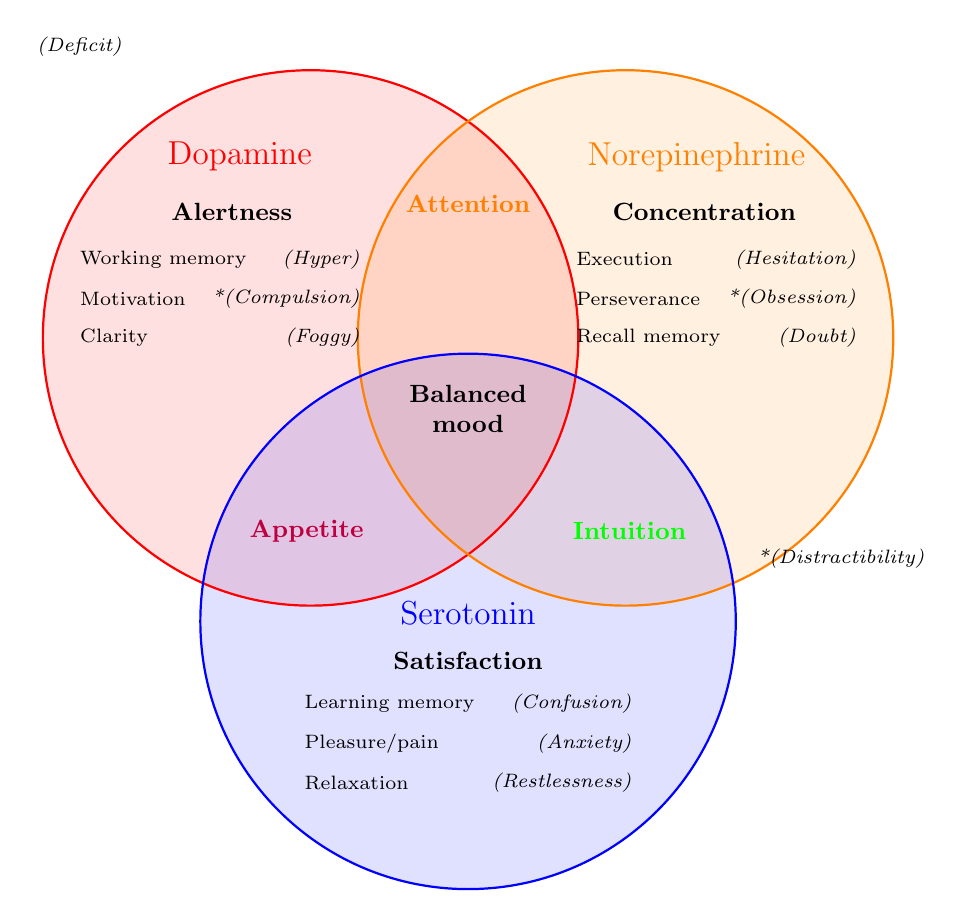
\begin{tikzpicture}[
  nt/.style={font=\large},
  fn/.style={font=\small\bfseries},
  row/.style={font=\scriptsize, anchor=west},
  def/.style={font=\scriptsize\itshape, anchor=east},
  ov/.style={font=\small\bfseries}
]
% the three monoamine circles
\fill[red, fill opacity=0.12] (-2,0.9) circle (3.4);
\fill[orange, fill opacity=0.12] (2,0.9) circle (3.4);
\fill[blue, fill opacity=0.12] (0,-2.7) circle (3.4);
\draw[red, thick] (-2,0.9) circle (3.4);
\draw[orange, thick] (2,0.9) circle (3.4);
\draw[blue, thick] (0,-2.7) circle (3.4);

% dopamine
\node[nt, red] at (-2.9,3.2) {Dopamine};
\node[fn] at (-3.0,2.5) {Alertness};
\node[row] at (-5.05,1.9) {Working memory};
\node[def] at (-1.25,1.9) {(Hyper)};
\node[row] at (-5.05,1.4) {Motivation};
\node[def] at (-1.25,1.4) {*(Compulsion)};
\node[row] at (-5.05,0.9) {Clarity};
\node[def] at (-1.25,0.9) {(Foggy)};

% norepinephrine
\node[nt, orange] at (2.9,3.2) {Norepinephrine};
\node[fn] at (3.0,2.5) {Concentration};
\node[row] at (1.25,1.9) {Execution};
\node[def] at (5.05,1.9) {(Hesitation)};
\node[row] at (1.25,1.4) {Perseverance};
\node[def] at (5.05,1.4) {*(Obsession)};
\node[row] at (1.25,0.9) {Recall memory};
\node[def] at (5.05,0.9) {(Doubt)};

% serotonin
\node[nt, blue] at (0,-2.6) {Serotonin};
\node[fn] at (0,-3.2) {Satisfaction};
\node[row] at (-2.2,-3.75) {Learning memory};
\node[def] at (2.2,-3.75) {(Confusion)};
\node[row] at (-2.2,-4.25) {Pleasure/pain};
\node[def] at (2.2,-4.25) {(Anxiety)};
\node[row] at (-2.2,-4.75) {Relaxation};
\node[def] at (2.2,-4.75) {(Restlessness)};

% overlaps
\node[ov, orange] at (0,2.6) {Attention};
\node[ov, purple] at (-2.05,-1.55) {Appetite};
\node[ov, green] at (2.05,-1.55) {Intuition};
\node[ov, align=center] at (0,0.0) {Balanced\\mood};

% legend notes from the slide
\node[font=\scriptsize\itshape, anchor=west] at (-5.6,4.6) {(Deficit)};
\node[font=\scriptsize\itshape, anchor=west] at (3.55,-1.9) {*(Distractibility)};
\end{tikzpicture}
